% arara: xelatex

\documentclass[11pt]{article}
\synctex=1

\usepackage{listings}
\usepackage{graphicx}
\setlength{\columnsep}{12.5pt}
\usepackage{caption}
\usepackage{cprotect}

\usepackage{xcolor}
\definecolor{mycolor}{HTML}{3CB5D6}

% Márgenes y espaciado
\usepackage[
	a4paper, % Tamaño del papel
	top=2.5cm, % Márgen superior
	bottom=2.5cm, % Márgen inferior
	left=2.25cm, % Márgen izquierdo
	right=2.25cm,
	footskip=1cm,
	headsep=0.5cm,
	headheight=1cm,
	%showframe
]{geometry}
\usepackage[nobottomtitles*]{titlesec}
\titlespacing*{\section}{0pt}{7.5pt}{8pt}

\usepackage{fontspec}
\usepackage[T1]{fontenc}

\setmainfont[
Path = /usr/share/fonts/TTF/,
ItalicFont = DejaVuSerif-Italic.ttf,
BoldFont = RobotoCondensed-Bold.ttf,
BoldItalicFont = RobotoCondensed-BoldItalic.ttf
]{DejaVuMathTeXGyre.ttf}

\setmonofont{Iosevka Fixed SS05}

\usepackage[spanish]{babel}

% Notas de colores
\usepackage{tcolorbox}
\tcbuselibrary{skins}
\newtcolorbox{mybox}[1]{
width=\textwidth,
colback=mycolor!10,
colbacktitle=mycolor,
boxrule=-0.1pt,
center,
fonttitle=\bfseries,
title={\hspace*{-8pt}#1}, % Sin indentación en el título
sharp corners
}

% Enlaces clicables
\usepackage[colorlinks=true, linkcolor=mycolor, urlcolor=mycolor]{hyperref}

\begin{document}

\pagestyle{empty}
\vspace*{.3\textheight}
{\hfill\Huge\itshape\textcolor{mycolor}{\textbf{Artix Linux}}\par}

{\hfill\Large Información útil\par}

\clearpage

\section{Compartir audio}

Al iniciar sesión se crea un \emph{micrófono virtual} con el que podemos combinar el audio de nuestro micrófono con el audio de las aplicaciones. De esta forma podemos compartir junto con nuestra pantalla, el audio de dicha retransmisión en aplicaciones que no tienen dicha funcionalidad.

\medskip
\noindent Para esto tendremos que elegir \emph{my-virtualmic} como nuestro micrófono predeterminado. Podemos añadir el audio de nuestro micrófono real y nuestras aplicaiones mediante el script \texttt{pipewire-virtualmic-select}.

\section{Cronie y scripts útiles}

El repositorio incluye una variedad de scripts para automatizar tareas. Por defecto no se usan, pero podemos hacer que se ejecuten de forma automática con \href{https://wiki.archlinux.org/title/cron}{crond}.

\subsection{convert-2m4a y convert-2mp3}

Estos scripts convierten toda la música del directorio que damos como primer argumento a formato \emph{.m4a} o \emph{.mp3} en un mirror que replica al estructura de los archivos en el directorio original.

\medskip
\noindent Si ejecutamos:
\begin{verbatim}
convert-2mp3 /musica/biblioteca /musica/mp3
\end{verbatim}
Toda la música de \path{/musica/biblioteca} se convertira en mp3 en la carpeta \path{/musica/mp3}
\begin{itemize}
	\item El script puede usarse con el flag \emph{-p} para convertir varios archivos de forma paralela, lo que reduce el tiempo necesario para la conversión de archivos, pero consume más recursos y probablemente ocupe todo el tiempo de CPU hasta que el script se termine de ejecutar.
	\item El script también puede usarse con el flag \emph{-l} lo que hará que además de convertir las canciones a otro formato, se busque la letra de la canción y se incluya dentro del archivo de audio.
\end{itemize}

\subsection{corruption-check}

Este script comprueba que no haya archivos corruptos en nuestra biblioteca de música, corrige falsos positivos de corrupción y nos escribe una lista con los archivos que no se pueden reproducir correctamente en \path{/tmp/corruption.log}. Necesita como argumento el directorio cuyos archivos de audio queremos analizar.

\subsection{exif-remove}

Este script necesita borra toda la información \href{https://en.wikipedia.org/wiki/Exif}{EXIF} de las imágenes que contiene el directorio que se le da como argumento.

\subsection{wake}

Este script comprueba si hay alguna máquina virtual en ejecución, y si no encuentra ninguna, suspende nuestro equipo y lo reanuda a las 7 de la mañana del día siguiente. Útil para ahorrar energía y no tener que preocuparte por suspender tu equipo, ni de encenderlo por las mañanas.

\medskip
El script te avisa de que el sistema se va suspender y pasados 10 minutos desde dicho aviso, suspende el sistema. \emph{Si el script se ejecuta pasándole el argumento ``now'', entonces el sistema se supenderá inmediatamente}.

\subsection{wakeme}

Este script funciona como un despertador, hace sonar el archivo de audio especificado hasta que le damos al un botón que apaga nuestra alarma.

\subsection{compressed-backup}

Este script crea un fichero comprimido \texttt{tar.gz} con una copia de seguridad del directorio que se le da por primer argumento en el directorio que se le da por segundo argumento. Además se encarga de borrar las copias de seguridad que tienen mas de un mes automáticamente.

\section{VFIO GPU passthrough}

Con VFIO (Virtual Function I/O) GPU passthrough podemos pasarle una tarjeta gráfica física a una máquina virtual. Lo que nos permite tener gráficos acelerados dentro de dicha máquina virtual.

\subsection{Pasos Iniciales}

\begin{itemize}
	\setlength\itemsep{-0.2em}
	\item Primero activamos \href{https://en.wikipedia.org/wiki/X86_virtualization#Intel-VT-d}{VT-d} o \href{https://en.wikipedia.org/wiki/X86_virtualization#AMD_virtualization_(AMD-V)}{AMD-v} \emph{dependiendo de si tenemos un procesador Intel o AMD}.
	\item Debemos de tener \href{https://en.wikipedia.org/wiki/Input\%E2\%80\%93output_memory_management_unit}{IOMMU} activado. En la mayoría de placas bases activar VT-d o AMD-v, también activa IOMMU.
	\item Debemos tener desactivado \href{https://en.wikipedia.org/wiki/UEFI#CSM_booting}{CSM (Compatibility Support Module)} en los ajustes de arranque de nuestra placa base.
\end{itemize}

\subsection{Pre-configurar el gestor de arranque}

El gestor de arranque \href{https://es.wikipedia.org/wiki/GNU_GRUB}{GNU GRUB}, es el programa que se encarga de cargar el kernel de nuestro sistema operativo.

\medskip
Para usar VFIO necesitamos configurar el arranque del kernel. Las opciones de configuración globales de GRUB están en \path{/etc/default/grub}

\medskip
Este archivo contiene las opciones de arranque del kernel en: \emph{GRUB\_CMDLINE\_LINUX}.

\begin{verbatim}
GRUB_CMDLINE_LINUX_DEFAULT="loglevel=3 quiet"
GRUB_CMDLINE_LINUX=""
\end{verbatim}

Tendremos que añadir las siguientes opciones:
\begin{itemize}
	\setlength\itemsep{-0.2em}
	\item \path{iommu=pt}
	\item \path{amd_iommu=on} o \path{intel_iommu=on}, dependiendo de si tenemos una cpu Intel o AMD.
	\item \path{video=efifb:off}
\end{itemize}

\begin{verbatim}
GRUB_CMDLINE_LINUX="intel_iommu=on iommu=pt video=efifb:off"
GRUB_CMDLINE_LINUX="amd_iommu=on iommu=pt video=efifb:off"
\end{verbatim}

Una vez editado el archivo, debemos actualizar nuestra configuración de GRUB con:

\begin{verbatim}
# grub-mkconfig -o /boot/grub/grub.cfg
\end{verbatim}

\subsection{Identificar el ID de nuestra gráfica y los grupos IOMMU}

Después de esto ya podemos asignar el driver VFIO a nuestra tarjeta gráfica para poder usarla en nuestra máquina virtual.

\vspace{5pt}

Necesitamos conocer el identificador de nuestra gráfica, podemos obtener esta informaciónejecutando en BASH:

\begin{verbatim}
shopt -s nullglob
for g in /sys/kernel/iommu_groups/*; do
    echo "IOMMU Group ${g##*/}:"
    for d in $g/devices/*; do
        echo -e "\t$(lspci -nns ${d##*/})"
    done;
done;
\end{verbatim}

\begin{lstlisting}[basicstyle=\scriptsize\ttfamily]
IOMMU Group 15:
  08:00.0 VGA compatible controller [0300]: NVIDIA TU116 [GeForce GTX 1660] [10de:21c4] (rev a1)
  08:00.1 Audio device [0403]: NVIDIA TU116 High Definition Audio Controller [10de:1aeb] (rev a1)
  08:00.2 USB controller [0c03]: NVIDIA Device [10de:1aec] (rev a1)
  08:00.3 Serial bus controller [0c80]: NVIDIA TU116 [GeForce GTX 1650] [10de:1aed] (rev a1)
\end{lstlisting}
Debemos añadir cada uno de los IDs de los dispositivos que se encuentran en el mismo grupo que nuestra gráfica (en nuestro ejemplo: \texttt{10de:21c4}, \texttt{10de:1aeb}, \texttt{10de:1aec} y \texttt{10de:1aed}) a nuestro archivo de configuración de GRUB, diciéndole que le asigne a estos dispositivos el driver vfio.

\begin{verbatim}
GRUB_CMDLINE_LINUX_DEFAULT="loglevel=3 quiet"
GRUB_CMDLINE_LINUX="amd_iommu=on iommu=pt video=efifb:off
vfio-pci.ids=10de:21c4,10de:1aeb,10de:1aec,10de:1aed"
\end{verbatim}

Ejecutamos de nuevo:
\begin{verbatim}
# grub-mkconfig -o /boot/grub/grub.cfg
\end{verbatim}

\subsection{Módulos del kernel}

Ahora cada vez que iniciemos nuestro ordenador el kernel intentará asignarle a esos dispositivos PCI el driver VFIO, pero el driver VFIO por defecto no se carga durante el arranque del sistema.

\medskip
Debemos de configurar nuestro kernel para que nuestra imagen de arranque incluya el driver VFIO, para poder asignarselo a nuestra gráfica.

\medskip
Para esto debemos editar \path{/etc/mkinitcpio.conf} y añadir los módulos del kernel que vamos a usar.

\begin{verbatim}
MODULES=( vfio_pci vfio vfio_iommu_type1 )
\end{verbatim}

Una vez editado nuestro archivo debemos regenerar el \href{https://en.wikipedia.org/wiki/Initial\_ramdisk}{initramfs} con:
\begin{verbatim}
# mkinitcpio -P
\end{verbatim}

Para comprobar que hemos seguido los pasos correctamente reiniciamos nuestro ordenador y cuando arranque de nuevo, ejecutamos:
\begin{verbatim}
# dmesg | grep -i vfio
\end{verbatim}

Si tenemos una salida parecida a:
\begin{lstlisting}[basicstyle=\small\ttfamily]
[3.416692] vfio_pci: add [10de:21c4[ffffffff:ffffffff]] class 0x000000/00000000
[3.433353] vfio_pci: add [10de:1aeb[ffffffff:ffffffff]] class 0x000000/00000000
[3.450019] vfio_pci: add [10de:1aec[ffffffff:ffffffff]] class 0x000000/00000000
[3.466953] vfio_pci: add [10de:1aed[ffffffff:ffffffff]] class 0x000000/00000000
\end{lstlisting}
donde podemos ver que el driver \path{vfio_pci} se ha cargado correctamente para nuestros dispositivos, entonces hemos realizado correctamente todos los pasos.

\subsection{Instalación del sistema operativo}

Ya tenemos lista nuestra gráfica para ser usada por nuestra máquina virtual, queda instalar nuestra máquina virtual y configurarla para usarla cómodamente.

\medskip
Descargamos la ISO de Windows 10 desde \href{https://www.microsoft.com/en-us/software-download/windows10ISO}{https://www.microsoft.com}, y los drivers que necesitará Windows desde \href{https://fedorapeople.org/groups/virt/virtio-win/direct-downloads/stable-virtio/virtio-win.iso}{https://fedorapeople.org}. Una vez descargadas las ISO, abrimos \emph{virt-manager} y creamos una máquina virtual:

\medskip
Asignamos la memoria RAM \emph{(8GB como mínimo)} a nuestra máquina virtual. Y en el último paso, elegimos \emph{customizar nuestra máquina virtual} antes de la instalación.

\begin{figure}[h]
	\centering
	\begin{minipage}[b]{0.4\textwidth}
		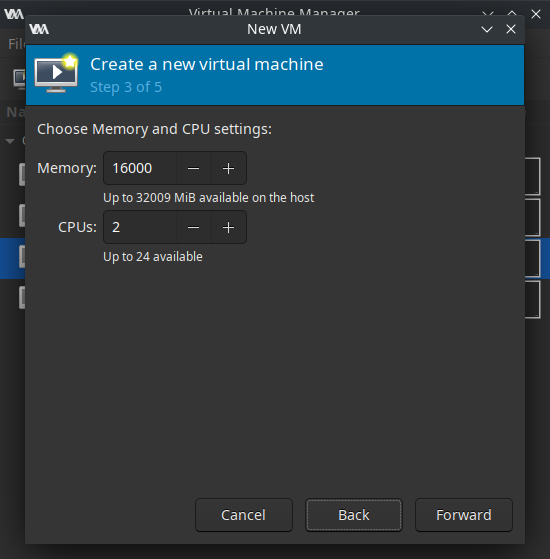
\includegraphics[width=0.9\textwidth]{images/vm-memory-setup.png}
	\end{minipage}
	\begin{minipage}[b]{0.4\textwidth}
		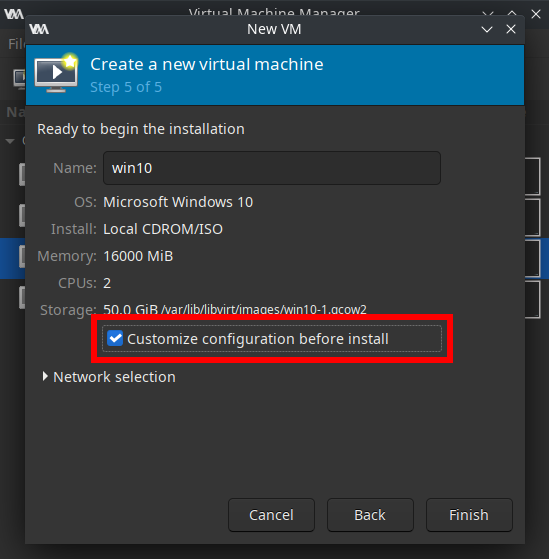
\includegraphics[width=0.9\textwidth]{images/vm-name.png}
	\end{minipage}
\end{figure}

Ahora deberás hacer las siguientes modificaciones:

\begin{itemize}
	\setlength\itemsep{-0.3em}
	\item Cambiar el chipset a \emph{Q35} y elegir el firmware \path{UEFI: x86_64: /usr/share/edk2/x64/OVMF_CODE.fd}
	\item Ajustar la  \emph{topología} del procesador de la siguiente manera:
	      \begin{itemize}
		      \item 1 \emph{socket}, tantos \emph{centros} comos núcleos tenga tu procesador y tantos \emph{hilos} como hilos tenga tu procesador por núcleo (ej. para un procesador de 8 núcleos, 16 hilos, elegiríamos: \emph{1 Socket, 8 Centros, 2 Hilos}).
	      \end{itemize}
	\item Cambiar el bus de nuestro disco virtual de \emph{SATA} a \emph{VirtIO}.
	\item Cambiar el modelo del \emph{NIC} a \emph{virtio}
	\item Añadir el ISO con los drivers virtio.
\end{itemize}

\clearpage

\begin{figure}[h!]
	\centering
	\begin{minipage}[b]{0.4965\textwidth}
		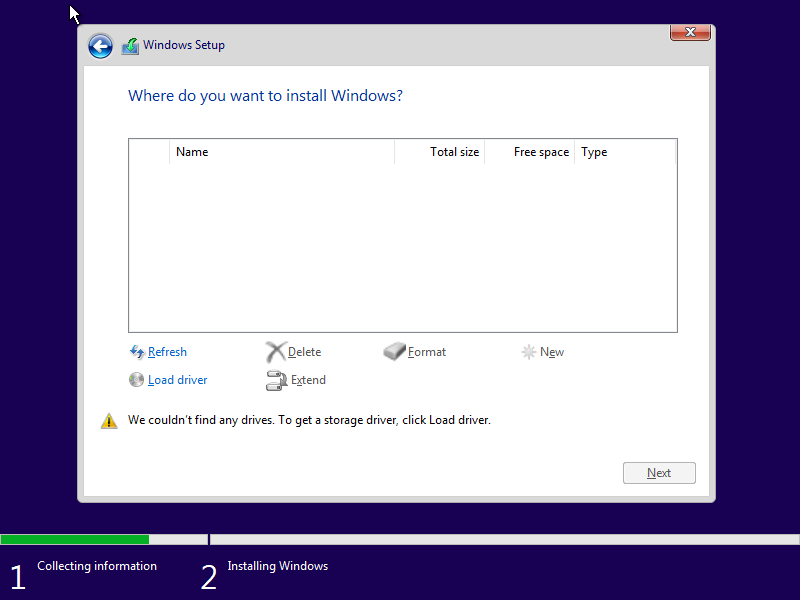
\includegraphics[width=\textwidth]{images/windows-setup-01.png}
	\end{minipage}
	\begin{minipage}[b]{0.4965\textwidth}
		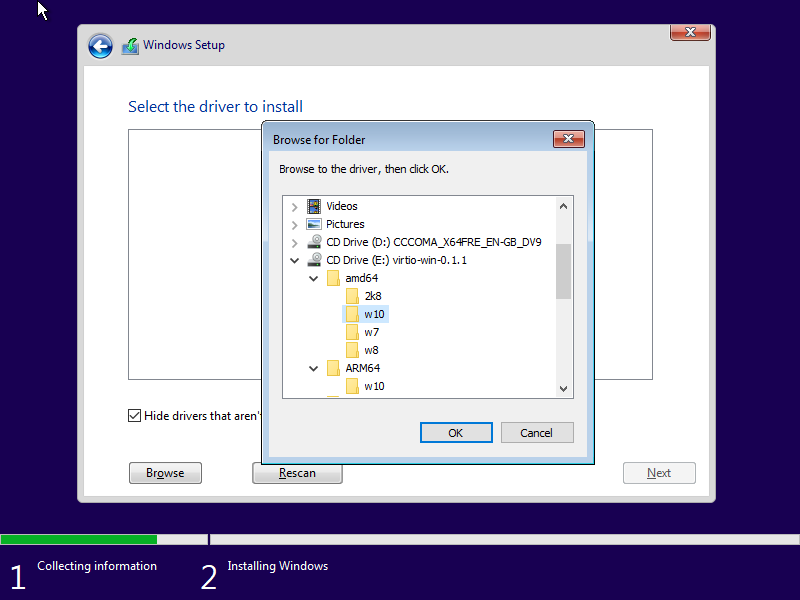
\includegraphics[width=\textwidth]{images/windows-setup-02.png}
	\end{minipage}
\end{figure}

Durante la instalación debemos cargar nuestro driver \emph{virtio} para que nuestro disco virtual sea detectado. \emph{Cuando la instalaciónd de windows finalize, apaga la máquina virtual.}

\begin{figure}[h!]
	\centering
	\begin{minipage}[b]{0.4965\textwidth}
		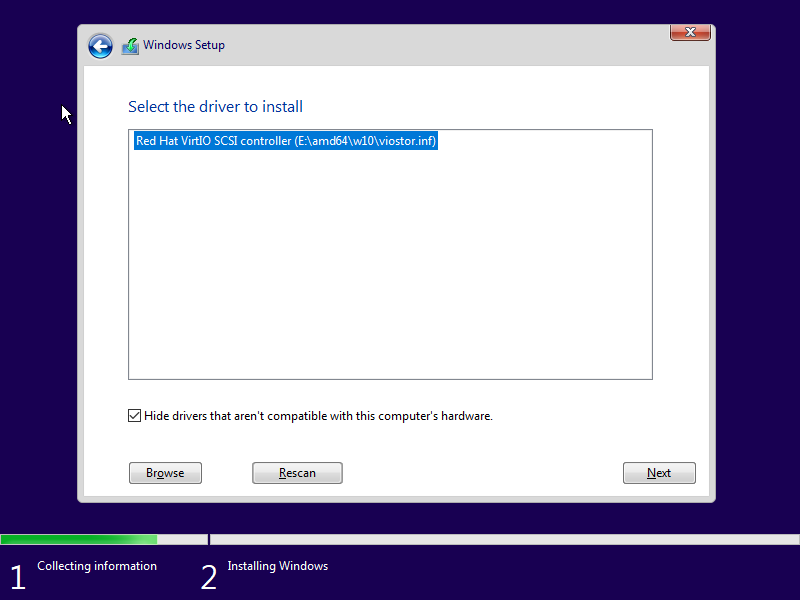
\includegraphics[width=\textwidth]{images/windows-setup-03.png}
	\end{minipage}
	\begin{minipage}[b]{0.4965\textwidth}
		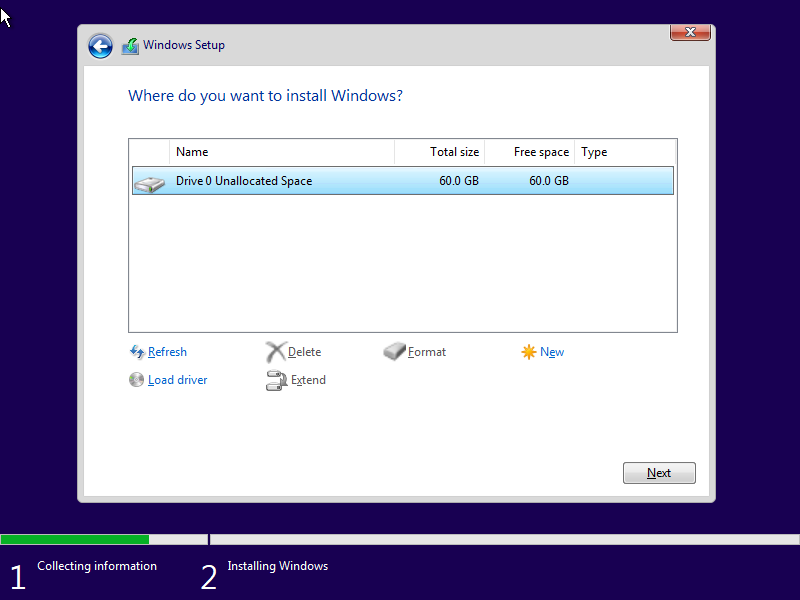
\includegraphics[width=\textwidth]{images/windows-setup-04.png}
	\end{minipage}
\end{figure}

\subsection{Looking Glass en el Host}

Para usar looking glass sin tener dos monitores, necesitamos un \href{https://www.amazon.com/s?k=display+dummy}{display dummy}.

\medskip
Looking Glass nos muestra una el output de nuestra gráfica con una latencia muy baja. Logra esto mandando la información a través de un archivo compartido entre máquina virtual y host.

Necesitamos instalar y configurar \emph{tmpfilesd} para que cada vez que iniciamos el sistema, se cree el archivo que compartido que Looking Glass necesita. Para eso ejecutamos los siguientes comandos:

\begin{verbatim}
echo "f /dev/shm/looking-glass 0660 $USER kvm -" | \
sudo tee -a /etc/tmpfiles.d/looking-glass.conf
\end{verbatim}
\begin{verbatim}
sudo pacman -Sy --noconfirm etmpfiles
\end{verbatim}

\subsection{Añadir Gráfica y Looking Glass en el Guest}

Ya tenemos casi todo listo, nos queda instalar los drivers de vídeo y Looking Glass en nuestra máquina virtual.

\medskip
Tenemos que añadir nuestra tarjeta gráfica a la máquina virtual. En \emph{``Añadir Dispositivo''}, buscamos la pestaña para añadir dispositivos PCI y añadimos la tarjeta gráfica.
Después debemos de configurar el servidor Spice para que use el puerto 6000 en vez de asignar un puerto automáticamente.

\begin{figure}[h!]
	\centering
	\begin{minipage}[b]{0.4965\textwidth}
		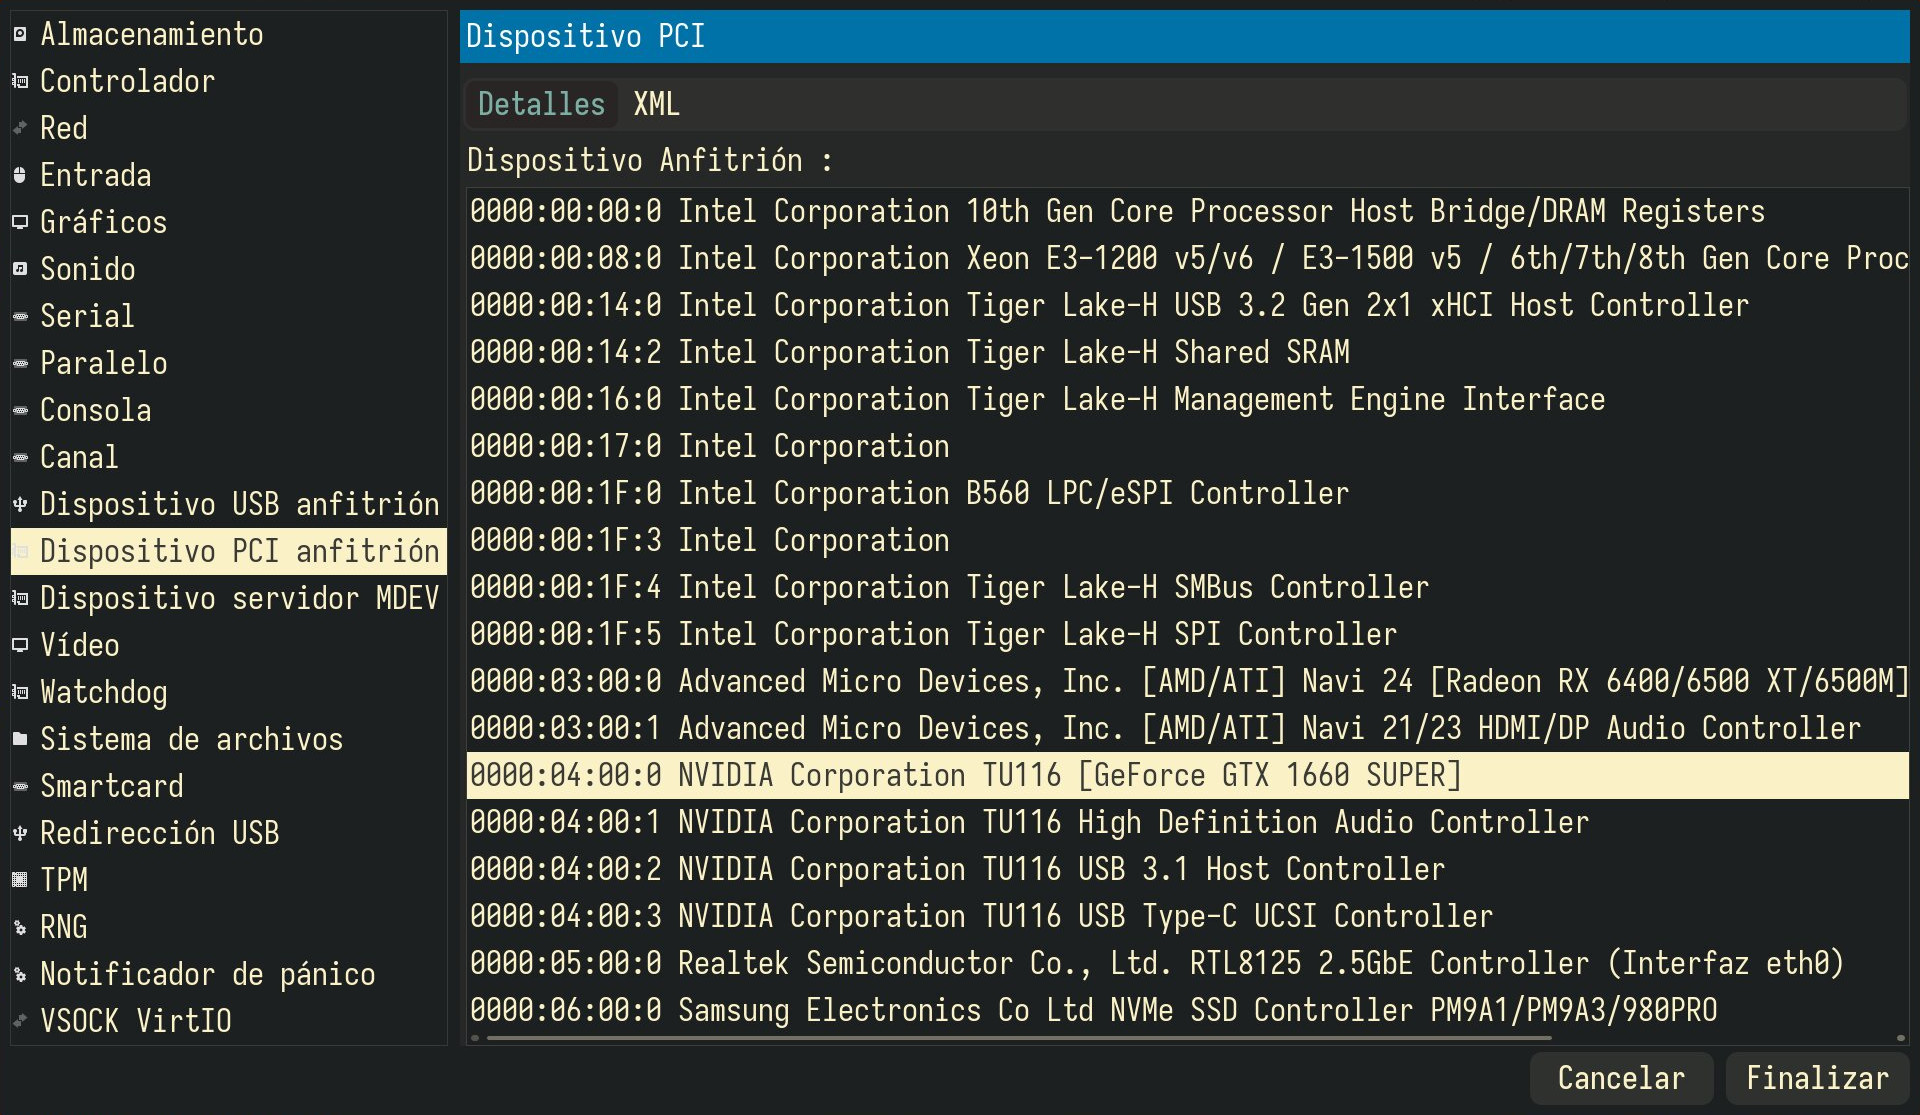
\includegraphics[height=0.6\textwidth,width=\textwidth]{images/card-add.jpg}
	\end{minipage}
	\begin{minipage}[b]{0.4965\textwidth}
		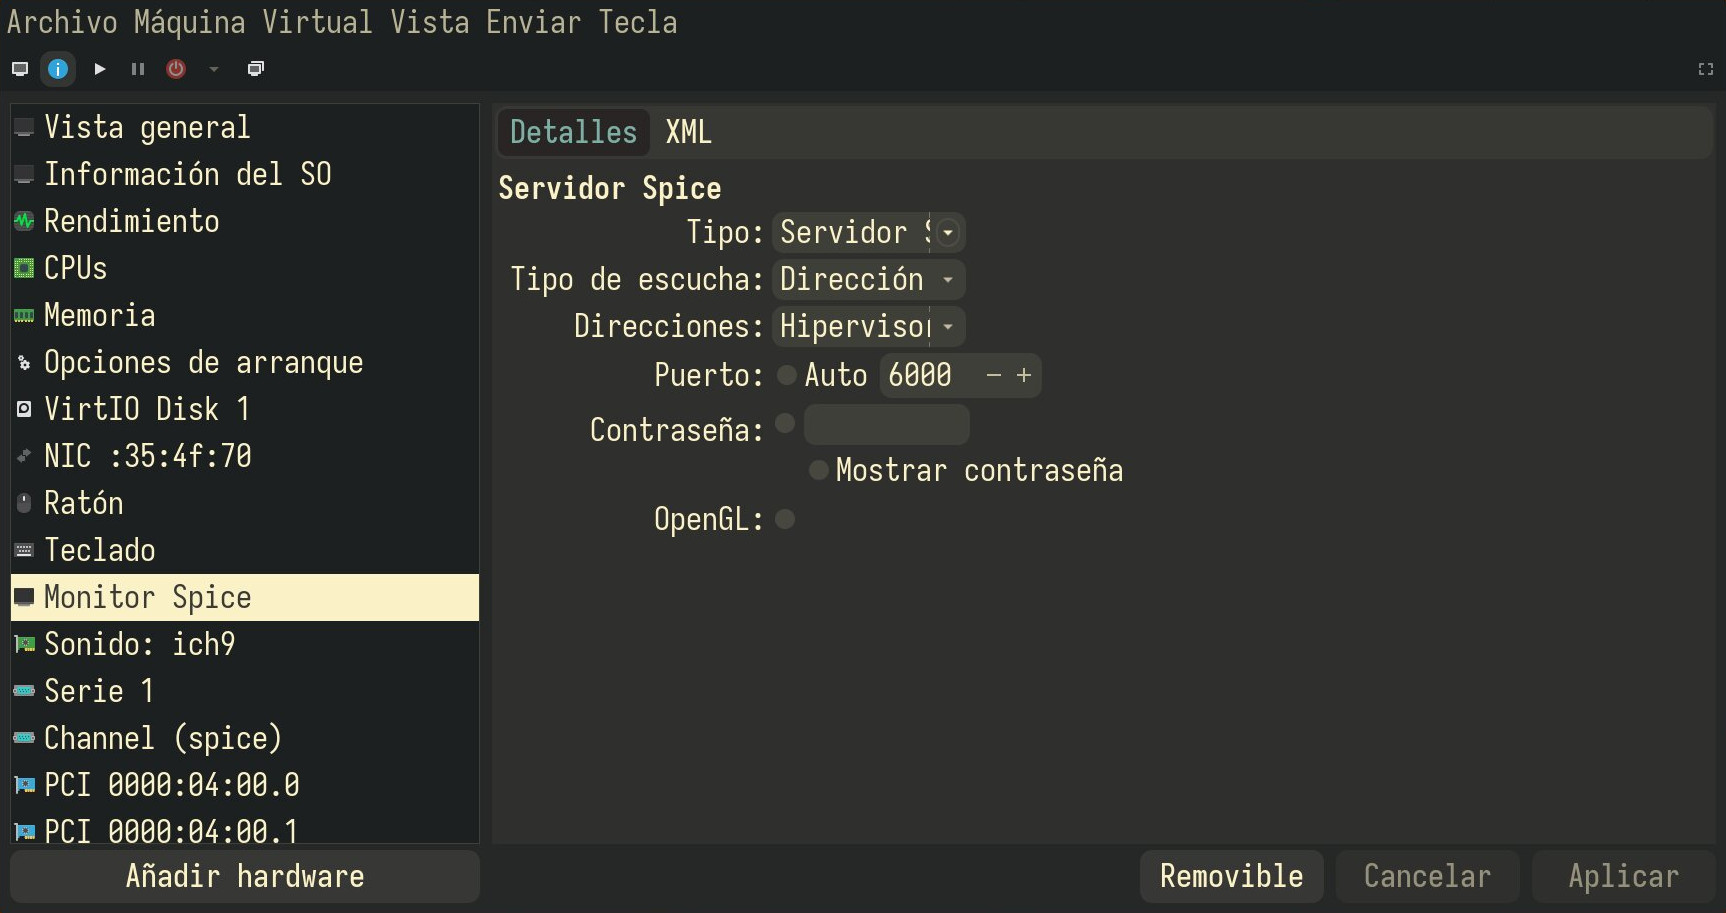
\includegraphics[height=0.6\textwidth,width=\textwidth]{images/spice-conf.jpg}
	\end{minipage}
\end{figure}

Ahora tenemos que activar la edición de XML en Virt-Manager \emph{(Editar, Preferencias)} y editar el código XML de nuestra máquina virtual añadiendo estas líneas justo después de las sección \texttt{</membaloon>}:

\begin{verbatim}
<shmem name='looking-glass'>
  <model type='ivshmem-plain'/>
  <size unit='M'>32</size>
</shmem>
\end{verbatim}

\begin{figure}[h!]
	\centering
	\begin{minipage}[b]{0.3285\textwidth}
		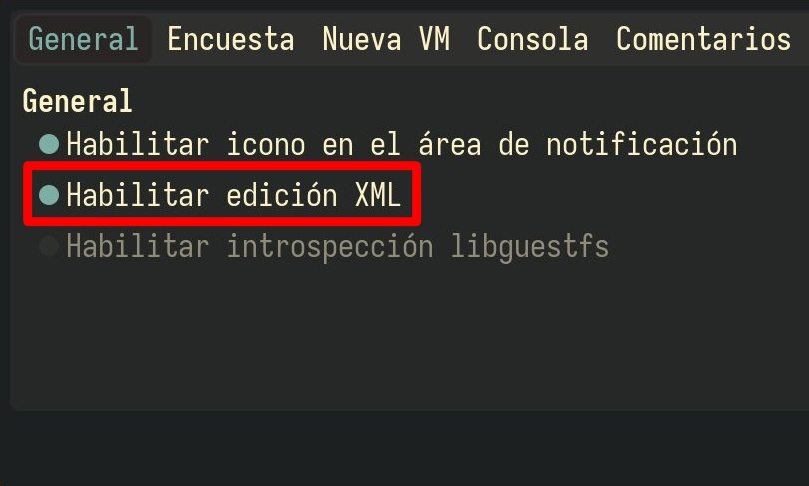
\includegraphics[height=0.6\textwidth,width=\textwidth]{images/xml-enable.jpg}
	\end{minipage}
	\begin{minipage}[b]{0.3285\textwidth}
		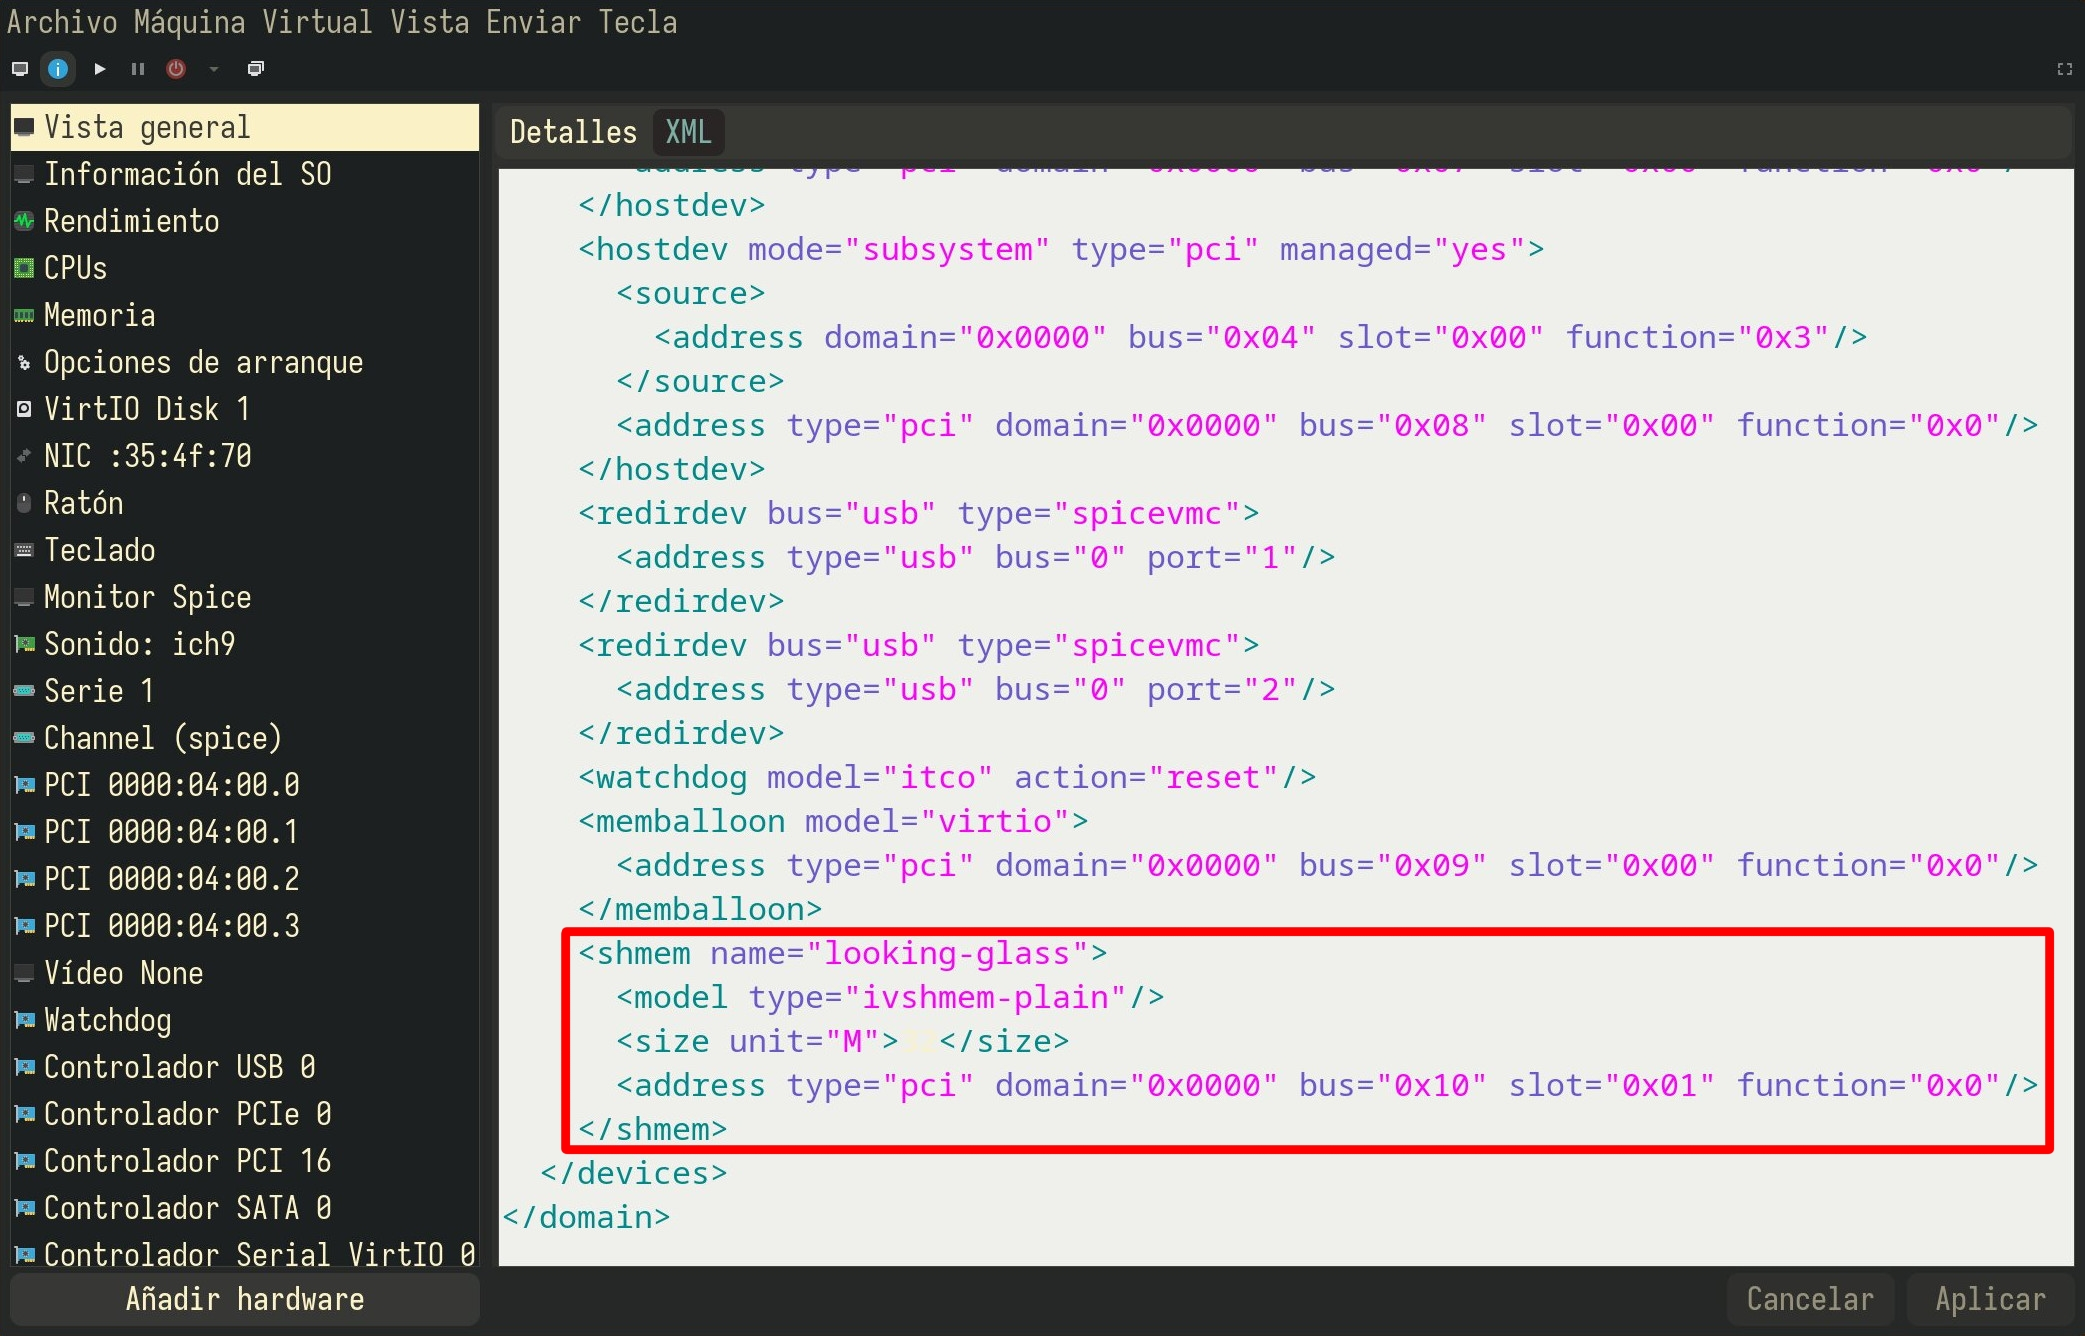
\includegraphics[height=0.6\textwidth,width=\textwidth]{images/xml-edit.jpg}
	\end{minipage}
	\begin{minipage}[b]{0.3285\textwidth}
		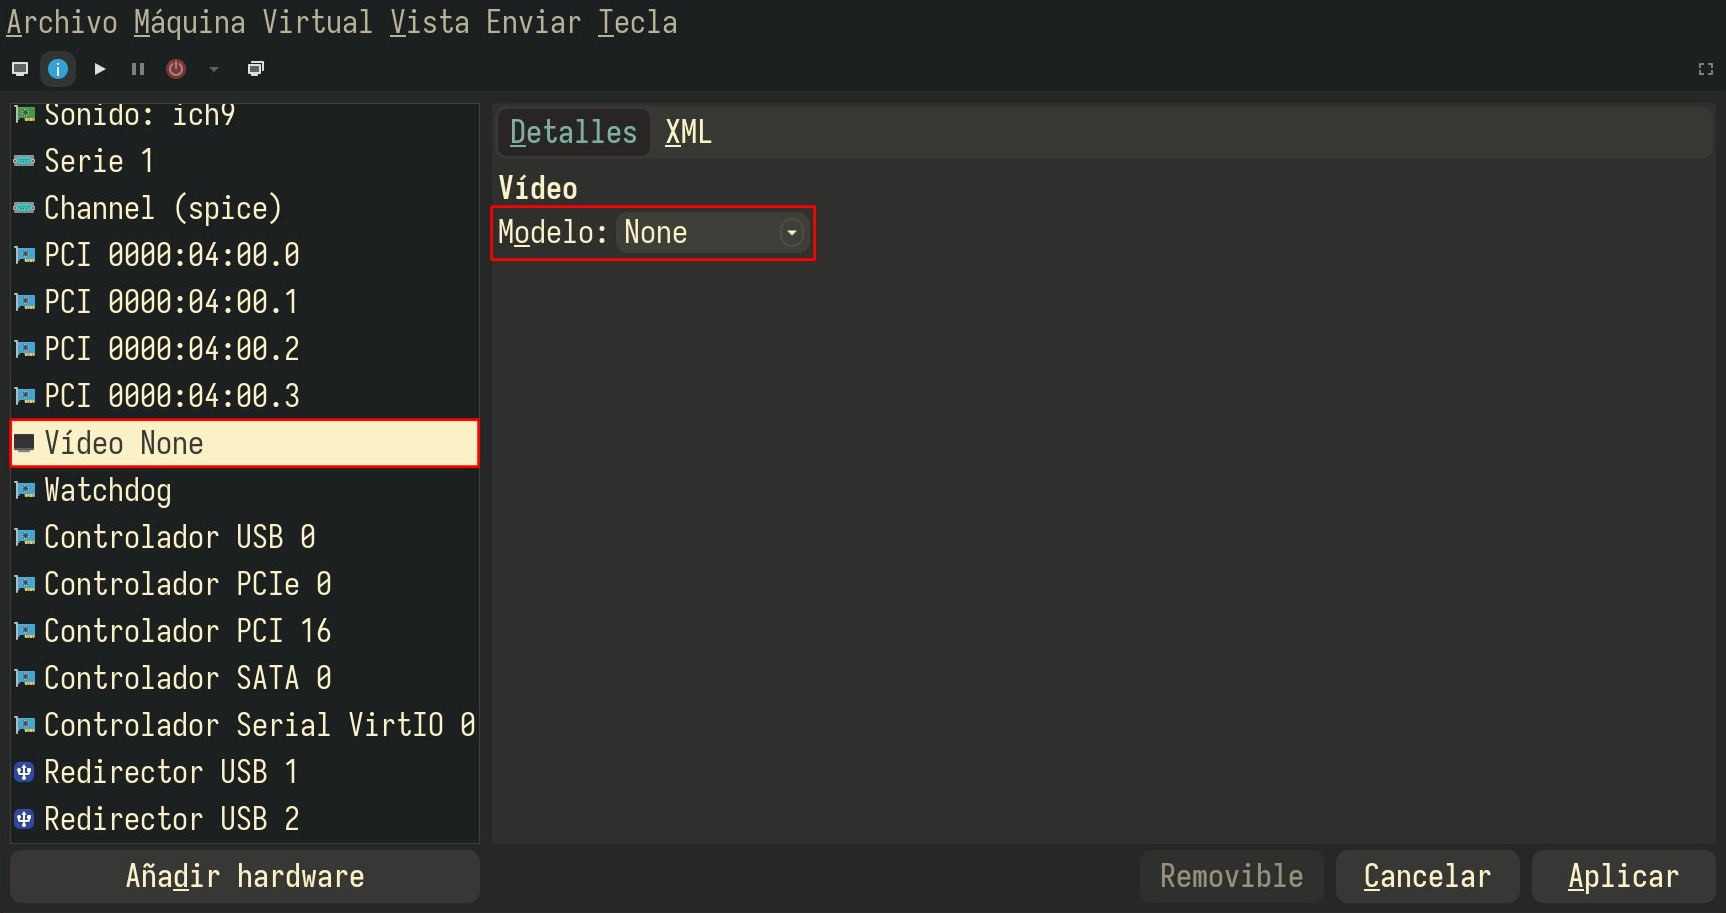
\includegraphics[height=0.6\textwidth,width=\textwidth]{images/video-none.jpg}
	\end{minipage}
\end{figure}

Iniciamos nuestra máquina virtual e instalamos nuestros drivers de \href{https://www.nvidia.es/Download/index.aspx?lang=es}{NVIDIA} o \href{https://www.amd.com/es/support}{AMD} y \href{https://looking-glass.io/downloads}{Looking Glass Host}.

\vspace{5pt}

Finalmente cambiamos el driver de vídeo de \emph{QXL} a \emph{None} y borramos el dispositivo de tableta táctil. La próxima vez que iniciemos la máquina virtual desde Virt-Manager podremos usarla através de Looking Glass con gráficos acelerados por hardware.

\noindent Para que esto funcione debemos reiniciar nuestro ordenador o ejecutar el comando.

\begin{verbatim}
sudo install -g kvm -o $(whoami) -m 0660 /dev/null /dev/shm/looking-glass
\end{verbatim}

\begin{mybox}{Nota}

	Para más información sobre como configurar un VFIO passthought puede consultar:

	\vspace{-7.5pt}

	\begin{itemize}
		\setlength\itemsep{-0.3em}
		\item \href{https://qqq.ninja/blog/post/vfio-on-arch/}
		      {https://qqq.ninja/blog/post/vfio-on-arch/}
		\item \href{https://gitlab.com/risingprismtv/single-gpu-passthrough/-/wikis/home}
		      {https://gitlab.com/risingprismtv/single-gpu-passthrough/-/wikis/home}
		\item \href{https://wiki.archlinux.org/title/PCI\_passthrough\_via\_OVMF}
		      {https://wiki.archlinux.org/title/PCI\_passthrough\_via\_OVMF}
	\end{itemize}
\end{mybox}

\section{VirtioFS}

Podemos usar virtiofs para compartir directorios del host con nuestra máquina virtual. Para ello, añadimos los directorios deseados desde Virt-Manager \emph(Añadir hardware, Sistema de archivos) eligiendo la \emph{ruta de origen} (la carpeta que queremos compartir) y la \emph{ruta objetivo} (el nombre con el que aparecerá en nuestra máquina invitada).

\medskip
Necesitamos también los controladores VirtIO y el software de integración con el host. Podemos instalarlos desde la ISO que descargamos en \href{https://fedorapeople.org/groups/virt/virtio-win/direct-downloads/stable-virtio/virtio-win.iso}{https://fedorapeople.org}. Esta contiene los instaladores necesarios \emph{(virtio-win-gt-x64.msi y virtio-win-guest-tools.exe)}

\medskip
Después de instalar los controladores, debemos instalar \href{https://github.com/winfsp/winfsp}{WinFSP} para poder montar sistemas de archivos VirtioFS. Podemos activar el servicio \emph{virtiofs} para que windows detecte nuestra carpeta compartida.

\subsubsection{Más de una carpeta}

Para compartir múltiples carpetas con nuestra máquina virtual, en lugar de utilizar el servicio \emph{virtiofs}, es necesario crear un script que monte las carpetas deseadas directamente en la máquina virtual.

\medskip
Para ello, primero ejecutamos desde cmd como Administrador:
\begin{center}
	{
		\fontsize{7.9}{9}\selectfont
		\texttt{
			\path{"}%
			C:\textbackslash Program Files (x86)\textbackslash WinFsp\textbackslash bin\textbackslash fsreg.bat%
			\path{"}
			virtiofs
			\path{"}%
			C:\textbackslash Program Files\textbackslash Virtio-Win\textbackslash VioFS\textbackslash virtiofs.exe%
			\path{"}
			\path{"}%
			-t\space \%1\space -m\space \%2%
			\path{"}
		}
	}
\end{center}

Una vez que tenemos todo instalado, creamos un script `.bat` que monte nuestras carpetas en la máquina invitada. Si tenemos dos carpetas cuyas rutas objetivo son ``documentos'' y ``videos'' y queremos montarlas en ``Y:'' y ``Z:'', respectivamente, podemos crear un script para montar ambas carpetas:
\begin{center}
	{
		\fontsize{9}{9}\selectfont
		\texttt{
			\path{"}%
			C:\textbackslash Program Files (x86)\textbackslash WinFsp\textbackslash bin\textbackslash launchctl-x64.exe%
			\path{"}
			start virtiofs documentos documentos Y:
		}
	}\\
	{
	\fontsize{9}{9}\selectfont
	\texttt{
		\path{"}%
		C:\textbackslash Program Files (x86)\textbackslash WinFsp\textbackslash bin\textbackslash launchctl-x64.exe%
		\path{"}
		start virtiofs videos videos Z:
	}
	}
\end{center}

\section{Conexión bridge y RDP}

Adicionalmente, podemos configurar nuestra máquina virtual para, a efectos prácticos, comportarse como un ordenador distinto en la red. En vez de usar un NAT y que nuestro host se encargue del re-direccionamiento al guest, podemos usar una conexión puente y hacer que nuestro router reconozca nuestra máquina virtual como un dipositivo distinto y le asigne su propia IP. De esta forma podemos abrir servicios desde nuestro guest y poder acceder a ellos.

\subsection{Creación de nuestra red puente}

Para crear nuestra conexión de puente, utilizaremos \emph{NetworkManager}:

\begin{itemize}
	\item Ejecutamos \texttt{nmtui}, seleccionamos \emph{Modificar una conexión} y elegimos añadir una nueva conexión \emph{(de tipo Puente)}.
	\item Debemos elegir que tarjeta de red queremos \emph{añadir} para la conexión puenteada. Elegiremos \emph{Ethernet}.
	\item Debemos eliminar la conexión Ethernet original de la lista de conexiones en (el host seguirá teniendo acceso a Internet; tanto la máquina anfitriona como la máquina invitada usarán la conexión de puente para acceder a Internet).
\end{itemize}

\subsection{Invitado con conexión puenteada}

Ahora tenemos que decirle a virt-manager que queremos usar nuestra conexión puenteada para la máquina virtual, podemos incluso borrar la red NAT \emph{`default'} si no tenemos ninguna otra máquina virtual que queramos conectar a Internet.

\medskip
Para usar la conexión puenteada en nuestra máquina virtual; en las propiedades de nuestra máquina virtual, cambiamos la \emph{`Fuente de red'} de nuestro NIC a la conexión puenteada.

Adicionalmente, podemos ajustar la dirección MAC y establecer una IP estática asociada a esa dirección MAC en nuestro router. Lo cual facilitará configurar servicios y acceder a nuestra máquina invitada desde la red.

\subsection{Configurar Escritorio remoto}

Ahora podemos configurar nuestra máquina invitada para acceder remotamente a ella mediante RDP, para ello en Windows \emph{(Sólo si tenemos Windows 10/11 Pro)} en Ajustes/Escritorio Remoto, activaremos el escritorio remoto.

Para conectaros a la máquina virtual de nuestra red debemos configurar el Firewall de nuestro guest para permitir las conexiones entrantes de RDP, para ello ejecutaremos este comando en cmd como Administrador:
\begin{centering}
	{
		\fontsize{9.75}{9}\selectfont
		\texttt{
			netsh advfirewall firewall add rule name=\path{"}RDP\path{"} protocol=TCP dir=in localport=3389 action=allow
		}
	}
\end{centering}

\medskip
Podemos conectarnos a nuestra máquina usando el script \texttt{rdp-connect}

\section{SSH}

Para conectarnos a nuestro equipo remotamente debemos configurar \href{https://es.wikipedia.org/wiki/OpenSSH}{OpenSSH}. Podemos configurar SSH de forma muy básica con el script:

\begin{verbatim}
ssh-configure
\end{verbatim}

Mi recomendación es no conformarse con esta configuración básica. Desactiva el login con el usuario root, desactiva el login por contraseña y usa claves públicas para conectarte.

\subsection{VNC através de SSH}

Podemos usar SSH y VNC para acceder a nuestro entorno gráfico de forma remota. Por defecto el script \texttt{autostart.sh} inicia un servidor \href{https://en.wikipedia.org/wiki/Virtual_Network_Computing}{VNC} para poder conectarnos remotamente a nuestro equipo. Para hacer uso del servidor VNC necesitamos usar \href{https://en.wikipedia.org/wiki/Tunneling_protocol}{tunneling} para que el tráfico de nuestro puerto 5900 \emph{(servidor vnc)} le llegue a nuestro equipo remoto:

\begin{verbatim}
ssh usuario@255.255.255.255 -L 5900:localhost:5900
\end{verbatim}

Sustituye \emph{usuario} por el usuario de tu máquina, y \emph{255.255.255.255} por la dirección IP de tu máquina. Para conectarte al equipo remotamente debes tener instalado algún cliente VNC, mi recomendación es \href{https://github.com/FreeRDP/Remmina}{remmina}.

\section{Firewall}

Para instalar el firewall ejecuta:

\begin{verbatim}
sudo sh -c 'pacman -Sy ufw-openrc; rc-update add ufw default; ufw enable'
\end{verbatim}

Podemos añadir unas reglas muy básicas a nuestro firewall \emph{(que se aplicarán cuando reiniciemos nuestro equipo)} con:

\begin{verbatim}
sudo ufw limit 22/tcp; sudo ufw allow 80/tcp
sudo ufw allow 443/tcp; sudo ufw allow syncthing
sudo ufw default deny incoming; sudo ufw default allow outgoing
\end{verbatim}

\begin{mybox}{Nota}
	Si configuraste ssh con \emph{ssh-configure} el firewall ya se configuró automáticamente
\end{mybox}

\section{Monitores de altas tasas de refresco}

Por defecto dwm actualiza el movimiento de las ventanas a 60 FPS. Si tienes un monitor de mas de 60 Hz esto puede hacer la experiencia de usar dwm insatisfactoria. Para cambiar este comportamiento, debes editar el archivo \emph{dwm.c}. En el encontrarás varias funciones con esta misma linea de código:

\begin{verbatim}
if ((ev.xmotion.time - lasttime) <= (1000 / 60))
\end{verbatim}

Deberás modificar el código según la tasa de refresco de tu monitor en cada aparición de esta linea. Por ejemplo, para un monitor de \emph{144 Hz}, la líneas a cambiar deberían verse así:

\begin{verbatim}
if ((ev.xmotion.time - lasttime) <= (1000 / 144))
\end{verbatim}

\section{Miscelánea}

\subsection*{Configuraciones locales}

Nuestra configuración de \texttt{zsh} tiene varios \emph{alias} configurados en:

\begin{center}
	\path{~/.config/zsh/aliasrc}
\end{center}

Para añadir alias fuera de la estructura del repositorio, de manera personal podemos crear un archivo con más funciones y abreviaciones en:

\begin{center}
	\path{~/.config/useralias}
\end{center}

\subsection*{Aviso de Uso}

Este proyecto es para uso personal. Se comparte con la intención de que pueda ser útil para otros, pero se proporciona tal cual, sin ninguna garantía. No se asume responsabilidad por ninguna pérdida de datos o problemas que puedan surgir del uso de este proyecto.

\end{document}
